\providecommand{\JVE}{\mathcal{J}_{\mathcal{VE}}}
\providecommand{\JVDbl}{\mathcal{J}_{v\mathcal{D}bl\mathcal{C}at}}
\providecommand{\Mof}[1]{\mathrm{M}_{#1}}

\section{模型无关\texorpdfstring{$\infty$}{∞}-范畴论的语言}\label{sec:language-for-model-independent-infinity-category-theory}

本节的目标是应用 Makkai 的\cref{thm:makkai-invariance}来证明：以\trVirtualEquipment{}的语言
写下的关于%
\trInfinityCategories{}的诸陈述——这一语言是为\cref{def:folds-signature-virtual-equipment}中引入的 FOLDS 签名
$\JVE$ 而定义的——在\trChangeOfModel{}之下不变。简单逆范畴
$\JVE$ 中的大部分复杂度，已然现身于%
\trVirtualDoubleCategory{}的 FOLDS 签名之中，我们将首先引入后者。

\begin{definition}\label{def:folds-signature-virtual-double-categories}
\trVirtualDoubleCategory{}的 FOLDS 签名 $\JVDbl$ 拥有分别对应于对象、竖直箭头、
水平\trModule{}以及诸%
$n$ 元\trCell（对每个 $n\ge 0$）的种类：
\end{definition}
\begin{center}
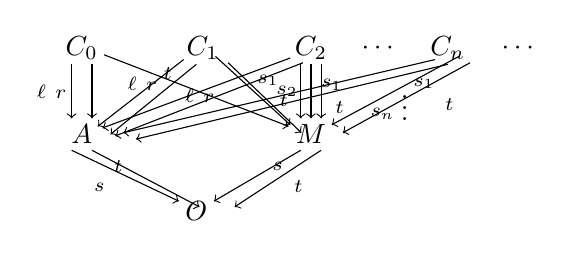
\begin{tikzpicture}[x=1.15em,y=1.15em]
  \node (C0) at (0,3.6)     {$C_{0}$};
  \node (C1) at (3.8,3.6)   {$C_{1}$};
  \node (C2) at (7.2,3.6)   {$C_{2}$};
  \node at (9.3,3.6)        {$\cdots$};
  \node (Cn) at (11.5,3.6)  {$C_{n}$};
  \node at (13.7,3.6)       {$\cdots$};
  \node (A) at (0,0.9)      {$A$};
  \node (M) at (7.2,0.9)    {$M$};
  \node (O) at (3.6,-1.5)   {$O$};
  \draw[->] (-0.32,3.1) -- (-0.32,1.4);
  \draw[->] (0.32,3.1)  -- (0.32,1.4);
  \node at (-0.95,2.25) {$\scriptstyle\ell\ r$};
  \draw[->] (3.2,3.25) -- (0.5,1.15);
  \draw[->] (3.6,3.1)  -- (0.9,0.9);
  \node at (1.9,2.5) {$\scriptstyle\ell\ r$};
  \draw[->] (6.55,3.3) -- (0.65,1.1);
  \draw[->] (6.95,3.15) -- (1.05,0.85);
  \node at (3.7,2.1) {$\scriptstyle\ell\ r$};
  \draw[->] (11.1,3.25) -- (1.3,0.95);
  \draw[->] (11.5,3.1)  -- (1.7,0.75);
  \draw[->] (0.7,3.4) -- (6.5,1.15);
  \node at (2.7,2.8) {$\scriptstyle t$};
  \draw[->] (4.2,3.35) -- (6.55,1.2);
  \node at (5.85,2.6) {$\scriptstyle s_{1}$};
  \draw[->] (4.6,3.15) -- (6.9,0.95);
  \node at (6.35,1.95) {$\scriptstyle t$};
  \draw[->] (6.88,3.1) -- (6.88,1.4);
  \draw[->] (7.2,3.1)  -- (7.2,1.4);
  \draw[->] (7.52,3.1) -- (7.52,1.4);
  \node at (6.45,2.25) {$\scriptstyle s_{2}$};
  \node at (7.85,2.45) {$\scriptstyle s_{1}$};
  \node at (8.1,1.75)  {$\scriptstyle t$};
  \draw[->] (11.85,3.35) -- (7.85,1.2);
  \node at (10.75,2.5) {$\scriptstyle s_{1}$};
  \node at (10.15,2.0) {$\scriptstyle\vdots$};
  \node at (9.45,1.55) {$\scriptstyle s_{n}$};
  \draw[->] (12.2,3.15) -- (8.2,0.95);
  \node at (11.55,1.85) {$\scriptstyle t$};
  \draw[->] (-0.32,0.4) -- (3.05,-1.2);
  \draw[->] (0.32,0.4)  -- (3.7,-1.38);
  \node at (1.15,-0.1) {$\scriptstyle t$};
  \node at (0.55,-0.75) {$\scriptstyle s$};
  \draw[->] (6.88,0.4) -- (4.15,-1.2);
  \draw[->] (7.52,0.4) -- (4.8,-1.38);
  \node at (6.15,-0.1) {$\scriptstyle s$};
  \node at (6.8,-0.75) {$\scriptstyle t$};
\end{tikzpicture}
\end{center}

每支箭头与每个模都拥有一个源对象与一个靶对象。每支 $n$ 元\trCell{}拥有一条左边
界箭头、一条右边界箭头、一个靶模以及 $n$ 个源模。此边界数据的源对象与靶对象
必须按由下列复合关系

\begin{equation*}
\begin{gathered}
s\cdot\ell = s\cdot s_{1} \qquad s\cdot r = t\cdot s_{n} \qquad t\cdot s_{k} = s\cdot s_{k+1},\quad 1\le k<n\\
t\cdot\ell = s\cdot t \qquad t\cdot r = t\cdot t
\end{gathered}
\end{equation*}

所指明的方式相容（于 $n\ge1$ 的情形\footnote{对零元\trCell，关系
$s\cdot\ell=s\cdot r$ 取代诸条涉及缺席源模的关系。}）。

另有两个种类 $I_{A}$ 与 $T$，分别参数化恒同竖直箭头与竖直箭头的复合，其复
合关系取自 1-范畴的签名：
\begin{equation*}
s\cdot i = t\cdot i \qquad s\cdot c = s\cdot\ell \qquad t\cdot c = t\cdot r \qquad t\cdot\ell = s\cdot r
\end{equation*}

每一类 $n$ 元\trCell{}都配备一个二元相等关系：
\begin{center}
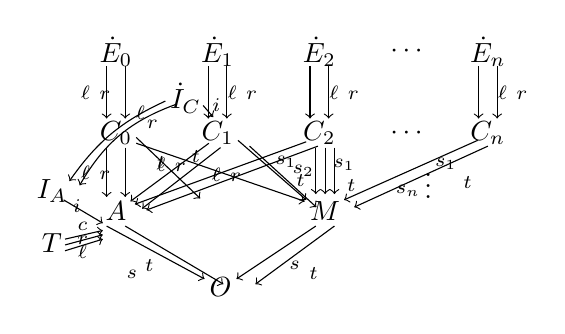
\begin{tikzpicture}[x=1.05em,y=1.05em]
  \node (E0) at (0,7.2)     {$\dot{E}_{0}$};
  \node (E1) at (3.5,7.2)   {$\dot{E}_{1}$};
  \node (E2) at (7.0,7.2)   {$\dot{E}_{2}$};
  \node at (10.0,7.2)       {$\cdots$};
  \node (En) at (12.8,7.2)  {$\dot{E}_{n}$};
  \node (IC) at (2.4,5.6)   {$\dot{I}_{C}$};
  \node (IA) at (-2.2,2.4)  {$I_{A}$};
  \node (T)  at (-2.2,0.6)  {$T$};
  \draw[->] (-0.32,6.7) -- (-0.32,4.9);
  \draw[->] (0.32,6.7)  -- (0.32,4.9);
  \node at (-0.7,5.8)  {$\scriptstyle\ell\ r$};
  \draw[->] (3.18,6.7) -- (3.18,4.9);
  \draw[->] (3.82,6.7) -- (3.82,4.9);
  \node at (4.35,5.8)  {$\scriptstyle\ell\ r$};
  \draw[->] (6.68,6.7) -- (6.68,4.9);
  \draw[->] (7.32,6.7) -- (7.32,4.9);
  \node at (7.85,5.8)  {$\scriptstyle\ell\ r$};
  \draw[->] (12.48,6.7) -- (12.48,4.9);
  \draw[->] (13.12,6.7) -- (13.12,4.9);
  \node at (13.65,5.8) {$\scriptstyle\ell\ r$};
  \draw[->] (3.0,5.35) -- (3.35,4.95);
  \node at (3.45,5.35) {$\scriptstyle i$};
  \draw[->] (1.7,5.5) to[bend right=15] (-1.6,2.75);
  \draw[->] (2.1,5.4) to[bend right=20] (-1.25,2.6);
  \node at (0.85,5.1) {$\scriptstyle\ell$};
  \node at (1.25,4.7) {$\scriptstyle r$};
  \node (C0) at (0,4.4)     {$C_{0}$};
  \node (C1) at (3.5,4.4)   {$C_{1}$};
  \node (C2) at (7.0,4.4)   {$C_{2}$};
  \node at (10.0,4.4)       {$\cdots$};
  \node (Cn) at (12.8,4.4)  {$C_{n}$};
  \draw[->] (0.7,4.25) -- (2.9,2.15);
  \node at (1.55,3.4) {$\scriptstyle t$};
  \draw[->] (-1.8,2.1) -- (-0.45,1.3);
  \node at (-1.35,1.9) {$\scriptstyle i$};
  \draw[->] (-1.75,0.75) -- (-0.45,1.05);
  \draw[->] (-1.75,0.55) -- (-0.45,0.9);
  \draw[->] (-1.75,0.35) -- (-0.45,0.75);
  \node at (-1.15,1.2) {$\scriptstyle c$};
  \node at (-1.15,0.72) {$\scriptstyle r$};
  \node at (-1.15,0.3) {$\scriptstyle \ell$};
  \draw[->] (-0.32,3.9) -- (-0.32,2.2);
  \draw[->] (0.32,3.9)  -- (0.32,2.2);
  \node at (-0.7,3.05) {$\scriptstyle\ell\ r$};
  \draw[->] (3.2,4.05) -- (0.5,2.05);
  \draw[->] (3.6,3.9)  -- (0.9,1.8);
  \node at (1.9,3.3) {$\scriptstyle\ell\ r$};
  \draw[->] (6.55,4.1) -- (0.65,1.95);
  \draw[->] (6.95,3.95) -- (1.05,1.75);
  \node at (3.8,2.95) {$\scriptstyle\ell\ r$};
  \draw[->] (0.7,4.05) -- (6.5,2.05);
  \node at (2.75,3.6) {$\scriptstyle t$};
  \draw[->] (4.2,4.15) -- (6.55,2.1);
  \node at (5.85,3.4) {$\scriptstyle s_{1}$};
  \draw[->] (4.6,3.95) -- (6.9,1.85);
  \node at (6.35,2.75) {$\scriptstyle t$};
  \draw[->] (6.88,3.9) -- (6.88,2.3);
  \draw[->] (7.2,3.9)  -- (7.2,2.3);
  \draw[->] (7.52,3.9) -- (7.52,2.3);
  \node at (6.45,3.1) {$\scriptstyle s_{2}$};
  \node at (7.85,3.3) {$\scriptstyle s_{1}$};
  \node at (8.1,2.6)  {$\scriptstyle t$};
  \draw[->] (12.45,4.15) -- (7.85,2.1);
  \node at (11.35,3.35) {$\scriptstyle s_{1}$};
  \node at (10.75,2.85) {$\scriptstyle\vdots$};
  \node at (10.05,2.4)  {$\scriptstyle s_{n}$};
  \draw[->] (12.8,3.95) -- (8.2,1.85);
  \node at (12.1,2.7) {$\scriptstyle t$};
  \node (A) at (0,1.7)    {$A$};
  \node (M) at (7.2,1.7)  {$M$};
  \node (O) at (3.6,-0.9) {$O$};
  \draw[->] (-0.32,1.2) -- (3.05,-0.62);
  \draw[->] (0.32,1.2)  -- (3.7,-0.8);
  \node at (1.15,-0.15) {$\scriptstyle t$};
  \node at (0.55,-0.45) {$\scriptstyle s$};
  \draw[->] (6.88,1.2) -- (4.15,-0.62);
  \draw[->] (7.52,1.2) -- (4.8,-0.8);
  \node at (6.15,-0.15) {$\scriptstyle s$};
  \node at (6.8,-0.45)  {$\scriptstyle t$};
\end{tikzpicture}
\end{center}

并满足一些等式，它们要求相等的\trCell{}必须具有相同的边界类型：
\begin{equation*}
\ell\cdot\ell = \ell\cdot r \qquad r\cdot\ell = r\cdot r \qquad t\cdot\ell = t\cdot r \qquad s_{k}\cdot\ell = s_{k}\cdot r
\end{equation*}

此外，在一个\trVirtualDoubleCategory{}中，每个模都拥有一支指定的恒同一元%
\trCell，其竖直源与靶为恒同箭头。关系符号 $\dot{I}_{C}$ 满足复合关系
\begin{equation*}
s\cdot i = t\cdot i \qquad \ell\cdot i = i\cdot\ell \qquad r\cdot i = i\cdot r
\end{equation*}
这些关系要求源模与靶模相重合，且左、右竖直箭头为恒同。

最后，对每一个分拆（partition）$n_{1}+\cdots+n_{k}=n$，都有一个 $(k+4)$ 元
关系符号 $\dot{T}_{n_{1},\ldots,n_{k}}$，其依赖关系如下图所示：
\begin{center}
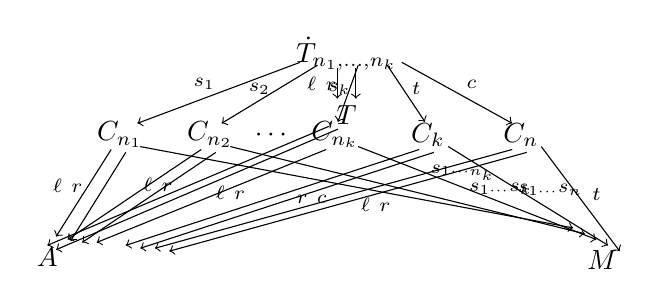
\begin{tikzpicture}[x=1.05em,y=1.05em]
  \node (Td) at (6.6,5.4) {$\dot{T}_{n_{1},\ldots,n_{k}}$};
  \node (Cn1) at (-1.2,2.6)  {$C_{n_{1}}$};
  \node (Cn2) at (1.9,2.6)   {$C_{n_{2}}$};
  \node at (4.0,2.6)          {$\cdots$};
  \node (Cnk) at (6.2,2.6)   {$C_{n_{k}}$};
  \node (Ck)  at (9.4,2.6)   {$C_{k}$};
  \node (Cn)  at (12.6,2.6)  {$C_{n}$};
  \draw[->] (5.0,5.1) -- (-0.6,3.0);
  \node at (1.7,4.35) {$\scriptstyle s_{1}$};
  \draw[->] (5.6,5.0) -- (2.3,3.0);
  \node at (3.6,4.2) {$\scriptstyle s_{2}$};
  \draw[->] (7.0,5.0) -- (6.3,3.05);
  \node at (6.35,4.2) {$\scriptstyle s_{k}$};
  \draw[->] (8.0,5.0) -- (9.3,3.05);
  \node at (9.0,4.2) {$\scriptstyle t$};
  \draw[->] (8.5,5.1) -- (12.3,3.0);
  \node at (10.9,4.35) {$\scriptstyle c$};
  \draw[->] (6.28,4.9) -- (6.28,3.85);
  \draw[->] (6.92,4.9) -- (6.92,3.85);
  \node at (5.75,4.35) {$\scriptstyle\ell\ r$};
  \node (T) at (6.6,3.3) {$T$};
  \draw[->] (-1.5,2.1) -- (-3.4,-0.9);
  \draw[->] (-1.0,2.0) -- (-2.9,-1.05);
  \node at (-3.0,0.85) {$\scriptstyle\ell\ r$};
  \draw[->] (1.6,2.1) -- (-3.0,-1.0);
  \draw[->] (2.1,2.0) -- (-2.5,-1.1);
  \node at (0.1,0.9) {$\scriptstyle\ell\ r$};
  \draw[->] (5.9,2.1) -- (-2.0,-1.1);
  \node at (2.6,0.6) {$\scriptstyle\ell\ r$};
  \draw[->] (9.1,2.1) -- (-1.0,-1.2);
  \draw[->] (9.6,2.0) -- (-0.5,-1.3);
  \node at (5.4,0.4) {$\scriptstyle r\ c$};
  \draw[->] (12.3,2.1) -- (0.0,-1.3);
  \draw[->] (12.8,2.0) -- (0.5,-1.4);
  \node at (7.6,0.2) {$\scriptstyle\ell\ r$};
  \draw[->] (-0.5,2.2) -- (14.4,-0.6);
  \draw[->] (2.6,2.2)  -- (14.8,-0.8);
  \node at (10.6,1.3) {$\scriptstyle s_{1\cdots n_{k}}$};
  \draw[->] (7.0,2.2) -- (15.2,-1.0);
  \node at (11.9,0.75) {$\scriptstyle s_{1\cdots}s_{k}$};
  \draw[->] (10.1,2.2) -- (15.6,-1.2);
  \node at (13.6,0.7) {$\scriptstyle s_{1\cdots}s_{n}$};
  \draw[->] (13.3,2.2) -- (16.0,-1.4);
  \node at (15.2,0.55) {$\scriptstyle t$};
  \draw[->] (6.0,2.9) -- (-3.7,-1.2);
  \draw[->] (6.3,2.8) -- (-3.4,-1.35);
  \node (A) at (-3.7,-1.6) {$A$};
  \node (M) at (15.4,-1.7) {$M$};
\end{tikzpicture}
\end{center}

并满足复合关系
\begin{equation*}
\begin{gathered}
s_{i}\cdot s_{j} = s_{n_{1}+\cdots+n_{j-1}+i}\cdot c \qquad
\ell\cdot\ell = \ell\cdot s_{1} \qquad
\ell\cdot r = r\cdot s_{k} \qquad
r\cdot s_{j} = \ell\cdot s_{j+1}\\
t\cdot s_{j} = s_{j}\cdot t \qquad
r\cdot\ell = \ell\cdot t \qquad
r\cdot r = r\cdot t\\
t\cdot t = t\cdot c \qquad
c\cdot\ell = \ell\cdot c \qquad
c\cdot r = r\cdot c
\end{gathered}
\end{equation*}

此处 $\dot{T}_{n_{1},\ldots,n_{k}}$ 是这样一个关系：它见证一支给定的 $n$ 元%
\trCell{}是 $k$ 支指定的源\trCell（元数（arity）分别为 $n_{1}$, \ldots, $n_{k}$）
复合入一支给定的靶 $k$ 元\trCell{}而成的复合。这样的复合还依赖于对竖直箭头的左、右交换
三角形的指定。

\begin{definition}\label{def:folds-signature-virtual-equipment}
\trVirtualEquipment{}的 FOLDS 签名 $\JVE$ 在\trVirtualDoubleCategory{}的
FOLDS 签名之上，添加两个额外的一元关系符号 $\dot{U}$ 与 $\dot{R}$，用以识别零
元单位\trModule{}与一元限制\trModule：
\end{definition}
\begin{center}
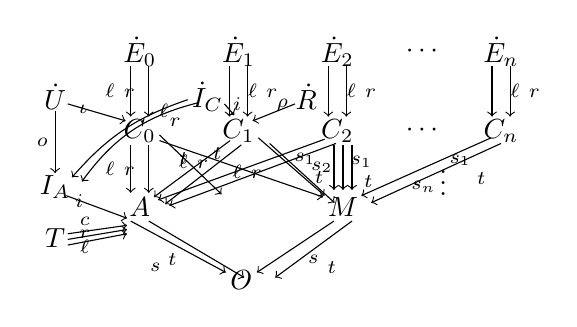
\begin{tikzpicture}[x=1.02em,y=1.02em]
  \node (U)  at (-3.0,5.6)  {$\dot{U}$};
  \node (E0) at (0,7.2)     {$\dot{E}_{0}$};
  \node (E1) at (3.5,7.2)   {$\dot{E}_{1}$};
  \node (E2) at (7.0,7.2)   {$\dot{E}_{2}$};
  \node at (10.0,7.2)       {$\cdots$};
  \node (En) at (12.8,7.2)  {$\dot{E}_{n}$};
  \node (IC) at (2.4,5.6)   {$\dot{I}_{C}$};
  \node (R)  at (5.9,5.6)   {$\dot{R}$};
  \node (IA) at (-3.0,2.4)  {$I_{A}$};
  \node (T)  at (-3.0,0.6)  {$T$};
  \draw[->] (-2.55,5.35) -- (-0.5,4.75);
  \node at (-2.0,5.15) {$\scriptstyle\iota$};
  \draw[->] (-3.0,5.1) -- (-3.0,2.9);
  \node at (-3.45,4.0) {$\scriptstyle o$};
  \draw[->] (5.5,5.35) -- (4.0,4.75);
  \node at (5.05,5.3) {$\scriptstyle\rho$};
  \draw[->] (-0.32,6.7) -- (-0.32,4.9);
  \draw[->] (0.32,6.7)  -- (0.32,4.9);
  \node at (-0.7,5.8)  {$\scriptstyle\ell\ r$};
  \draw[->] (3.18,6.7) -- (3.18,4.9);
  \draw[->] (3.82,6.7) -- (3.82,4.9);
  \node at (4.35,5.8)  {$\scriptstyle\ell\ r$};
  \draw[->] (6.68,6.7) -- (6.68,4.9);
  \draw[->] (7.32,6.7) -- (7.32,4.9);
  \node at (7.85,5.8)  {$\scriptstyle\ell\ r$};
  \draw[->] (12.48,6.7) -- (12.48,4.9);
  \draw[->] (13.12,6.7) -- (13.12,4.9);
  \node at (13.65,5.8) {$\scriptstyle\ell\ r$};
  \draw[->] (3.0,5.35) -- (3.35,4.95);
  \node at (3.45,5.35) {$\scriptstyle i$};
  \draw[->] (1.7,5.5) to[bend right=15] (-2.4,2.75);
  \draw[->] (2.1,5.4) to[bend right=20] (-2.05,2.6);
  \node at (0.85,5.1) {$\scriptstyle\ell$};
  \node at (1.25,4.7) {$\scriptstyle r$};
  \node (C0) at (0,4.4)     {$C_{0}$};
  \node (C1) at (3.5,4.4)   {$C_{1}$};
  \node (C2) at (7.0,4.4)   {$C_{2}$};
  \node at (10.0,4.4)       {$\cdots$};
  \node (Cn) at (12.8,4.4)  {$C_{n}$};
  \draw[->] (0.7,4.25) -- (2.9,2.15);
  \node at (1.55,3.4) {$\scriptstyle t$};
  \draw[->] (-2.6,2.1) -- (-0.45,1.3);
  \node at (-2.15,1.9) {$\scriptstyle i$};
  \draw[->] (-2.55,0.75) -- (-0.45,1.05);
  \draw[->] (-2.55,0.55) -- (-0.45,0.9);
  \draw[->] (-2.55,0.35) -- (-0.45,0.75);
  \node at (-1.95,1.2) {$\scriptstyle c$};
  \node at (-1.95,0.72) {$\scriptstyle r$};
  \node at (-1.95,0.3) {$\scriptstyle \ell$};
  \draw[->] (-0.32,3.9) -- (-0.32,2.2);
  \draw[->] (0.32,3.9)  -- (0.32,2.2);
  \node at (-0.7,3.05) {$\scriptstyle\ell\ r$};
  \draw[->] (3.2,4.05) -- (0.5,2.05);
  \draw[->] (3.6,3.9)  -- (0.9,1.8);
  \node at (1.9,3.3) {$\scriptstyle\ell\ r$};
  \draw[->] (6.55,4.1) -- (0.65,1.95);
  \draw[->] (6.95,3.95) -- (1.05,1.75);
  \node at (3.8,2.95) {$\scriptstyle\ell\ r$};
  \draw[->] (0.7,4.05) -- (6.5,2.05);
  \node at (2.75,3.6) {$\scriptstyle t$};
  \draw[->] (4.2,4.15) -- (6.55,2.1);
  \node at (5.85,3.4) {$\scriptstyle s_{1}$};
  \draw[->] (4.6,3.95) -- (6.9,1.85);
  \node at (6.35,2.75) {$\scriptstyle t$};
  \draw[->] (6.88,3.9) -- (6.88,2.3);
  \draw[->] (7.2,3.9)  -- (7.2,2.3);
  \draw[->] (7.52,3.9) -- (7.52,2.3);
  \node at (6.45,3.1) {$\scriptstyle s_{2}$};
  \node at (7.85,3.3) {$\scriptstyle s_{1}$};
  \node at (8.1,2.6)  {$\scriptstyle t$};
  \draw[->] (12.45,4.15) -- (7.85,2.1);
  \node at (11.35,3.35) {$\scriptstyle s_{1}$};
  \node at (10.75,2.85) {$\scriptstyle\vdots$};
  \node at (10.05,2.4)  {$\scriptstyle s_{n}$};
  \draw[->] (12.8,3.95) -- (8.2,1.85);
  \node at (12.1,2.7) {$\scriptstyle t$};
  \node (A) at (0,1.7)    {$A$};
  \node (M) at (7.2,1.7)  {$M$};
  \node (O) at (3.6,-0.9) {$O$};
  \draw[->] (-0.32,1.2) -- (3.05,-0.62);
  \draw[->] (0.32,1.2)  -- (3.7,-0.8);
  \node at (1.15,-0.15) {$\scriptstyle t$};
  \node at (0.55,-0.45) {$\scriptstyle s$};
  \draw[->] (6.88,1.2) -- (4.15,-0.62);
  \draw[->] (7.52,1.2) -- (4.8,-0.8);
  \node at (6.15,-0.15) {$\scriptstyle s$};
  \node at (6.8,-0.45)  {$\scriptstyle t$};
\end{tikzpicture}
\end{center}

单位模的左、右竖直箭头是同一对象上的恒同，这由如下复合关系表达：
\begin{equation*}
\ell\cdot\iota = i\cdot o = r\cdot\iota.
\end{equation*}

一元限制\trCell{}的边界不施加任何复合关系。这一数据便构成了 Cruttwell 与
Shulman 意义下\trVirtualEquipment{}的 FOLDS 签名。

任何\trVirtualEquipment{}都以一种朴素的（naïve）方式定义一个 $\JVE$-结构：取函子
$\JVE\to\mathcal{S}et$，令其把每个种类或关系符号送到其预期的解释（interpretation）。
\footnote{由于最令人感兴趣的虚拟装备都是大的，相应的 $\JVE$-结构也是大的。}
但正如 2-范畴的情形那样，对象 $I_{A}$ 与 $T$ 并非\trVirtualEquipment{}的
FOLDS 签名中的关系符号，故与这两个对象相关联的匹配映射无须
是\trMonomorphism。这使得我们有余地以一种更为「饱和的」方式把一
个\trVirtualEquipment{}转换为一个 $\JVE$-结构。事实上，与\cref{exa:pseudo-comma-2-category}和%
\cref{ex:naive-not-j-equivalent}相类比，为了证明我们想要的结果之一——%
\trVirtualEquipment{}间的一个\trBiequivalence{}给出（\cref{def:j-equivalent-in-context}意义下的）
一个 $\JVE$-等价——必须以这
种方式对与\trVirtualEquipment{}相关联的 $\JVE$-结构作「饱和化」（saturate）。
与\cref{exa:e-d-functors-2cat}中一样，也可以这样来定义与一个\trVirtualEquipment{}相关联的「饱
和的」$\JVE$-结构：定义一个从 $\JVE$ 到「\trVirtualEquipment{}及其保持结构的
函子」之\trCategory{}的相应反变函子；但在此情形，出现在指标图中的那些%
\trVirtualEquipment{}描述起来更为复杂，因此我们转而直接描述这一结构。

\begin{recall}\label{rec:vertical-two-category}
回顾第 8 章中的\cref{prop:vertical-two-category}：任何\trVirtualEquipment{}%
都包含一个%
\emph{竖直 2-范畴}（vertical 2-category），其对象是该\trVirtualEquipment{}的
对象，其箭头是竖直箭头，其 2-\trCell{}则是如下所示的那些一元\trCell：
\begin{rveq}\label{eq:vertical-2-category-unary-cell}
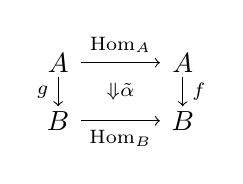
\begin{tikzpicture}[x=1.5em,y=1.5em]
  \node at (0,1.4) {$A$};
  \node at (3.0,1.4) {$A$};
  \draw[->] (0.55,1.4) -- node[above]{$\scriptstyle\mathrm{Hom}_{A}$} (2.45,1.4);
  \draw[->] (0,1.05) -- node[left]{$\scriptstyle g$} (0,0.35);
  \draw[->] (3.0,1.05) -- node[right]{$\scriptstyle f$} (3.0,0.35);
  \node at (1.5,0.7) {$\scriptstyle\Downarrow\tilde{\alpha}$};
  \node at (0,0) {$B$};
  \node at (3.0,0) {$B$};
  \draw[->] (0.55,0) -- node[below]{$\scriptstyle\mathrm{Hom}_{B}$} (2.45,0);
\end{tikzpicture}
\end{rveq}
其水平边界箭头由诸单位模给出。令人混淆的是，2-\trCell{}的「水平复合」由\trVirtualEquipment{}中一元\trCell{}%
的竖直复合来承载，而 2-\trCell{}的「竖直复合」则由第 8 章中的%
\cref{def:horizontal-composite-cells}所定义的水平复合运算来承载。特别地，当
竖直 2-范畴中的一元\trCell{}在 2-范畴中 2-\trCell{}的通常意义下可逆时——亦即
在\trVirtualEquipment{}中单位模之间的一元\trCell{}的水平复合运算意义下可逆时
——我们称其为「可逆的」；注意，竖直 2-范畴中一支可逆\trCell{}的竖直边界
1-\trCell{}无须在任何意义下可逆。

事实上，第 8 章中的\cref{def:horizontal-composite-cells}所描述的构造可作如
下推广。给定\trVirtualEquipment{}中的任意一支\trCell{}与一对竖直 2-范畴中的%
\trCell，如下所示
\begin{rveq}\label{eq:horizontal-composite-data}
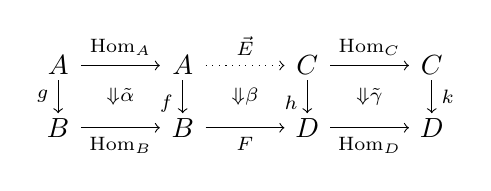
\begin{tikzpicture}[x=1.5em,y=1.5em]
  \node at (0,1.5)   {$A$};
  \node at (3.0,1.5) {$A$};
  \node at (6.0,1.5) {$C$};
  \node at (9.0,1.5) {$C$};
  \draw[->] (0.55,1.5) -- node[above]{$\scriptstyle\mathrm{Hom}_{A}$} (2.45,1.5);
  \draw[->,dotted] (3.55,1.5) -- node[above]{$\scriptstyle\vec{E}$} (5.45,1.5);
  \draw[->] (6.55,1.5) -- node[above]{$\scriptstyle\mathrm{Hom}_{C}$} (8.45,1.5);
  \draw[->] (0,1.15) -- node[left]{$\scriptstyle g$} (0,0.35);
  \node at (1.5,0.75) {$\scriptstyle\Downarrow\tilde{\alpha}$};
  \draw[->] (3.0,1.15) -- node[left,pos=0.7]{$\scriptstyle f$} (3.0,0.35);
  \node at (4.5,0.75) {$\scriptstyle\Downarrow\beta$};
  \draw[->] (6.0,1.15) -- node[left,pos=0.7]{$\scriptstyle h$} (6.0,0.35);
  \node at (7.5,0.75) {$\scriptstyle\Downarrow\tilde{\gamma}$};
  \draw[->] (9.0,1.15) -- node[right]{$\scriptstyle k$} (9.0,0.35);
  \node at (0,0)   {$B$};
  \node at (3.0,0) {$B$};
  \node at (6.0,0) {$D$};
  \node at (9.0,0) {$D$};
  \draw[->] (0.55,0) -- node[below]{$\scriptstyle\mathrm{Hom}_{B}$} (2.45,0);
  \draw[->] (3.55,0) -- node[below]{$\scriptstyle F$} (5.45,0);
  \draw[->] (6.55,0) -- node[below]{$\scriptstyle\mathrm{Hom}_{D}$} (8.45,0);
\end{tikzpicture}
\end{rveq}
存在唯一的一支「水平复合」\trCell，其边界为
\begin{rveq}\label{eq:horizontal-composite-cell}
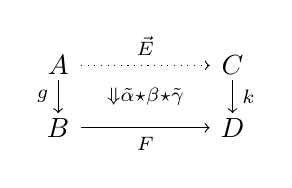
\begin{tikzpicture}[x=1.5em,y=1.5em]
  \node at (0,1.5) {$A$};
  \node at (4.2,1.5) {$C$};
  \draw[->,dotted] (0.55,1.5) -- node[above]{$\scriptstyle\vec{E}$} (3.65,1.5);
  \draw[->] (0,1.15) -- node[left]{$\scriptstyle g$} (0,0.35);
  \node at (2.1,0.75) {$\scriptstyle\Downarrow\tilde{\alpha}\star\beta\star\tilde{\gamma}$};
  \draw[->] (4.2,1.15) -- node[right]{$\scriptstyle k$} (4.2,0.35);
  \node at (0,0) {$B$};
  \node at (4.2,0) {$D$};
  \draw[->] (0.55,0) -- node[below]{$\scriptstyle F$} (3.65,0);
\end{tikzpicture}
\end{rveq}
并满足粘贴等式 \eqref{eq:horizontal-composite-pasting} 的类似物，后者是相对
于第 8 章中的\cref{lem:composites-with-units}的诸典范复合胞腔而定义的。在下
文中，我们将滥用记号，写出一个形如
\eqref{eq:horizontal-composite-data}的表达式来指称复合胞腔
\eqref{eq:horizontal-composite-cell}。

在\trInfinityCosmos{} $\mathcal{K}$ 中模的\trVirtualEquipment{}
$\Mod(\mathcal{K})$ 里，
这个竖直 2-范畴同构于\trHomotopyTwoCategory{} $\mathfrak{h}\mathcal{K}$。由
于我们打算在下述构造中应用于这一语境，故当从\trHomotopyTwoCategory{}借来的
记号更易读时，我们便借用之——例如，对竖直 2-范畴中右边界为 $f$、左边界为 $g$
的一支一元胞腔 \eqref{eq:vertical-2-category-unary-cell}，写作
$\alpha\colon f\Rightarrow g$。
\end{recall}

\begin{definition}\label{def:ve-structure-of-virtual-equipment}
对任何\trVirtualEquipment{} $\C$，都存在一个 $\JVE$-结构 $\Mof{\C}$，其中：
\begin{itemize}
\item 集合 $\Mof{\C}O$、$\Mof{\C}A$、$\Mof{\C}M$ 与诸 $\Mof{\C}C_{n}$（对每
个 $n\ge 0$）按其朴素解释分别取为 $\C$ 中对象、竖直箭头、水平\trModule{}与
$n$ 元\trCell{}的集合；
\item 诸二元关系 $\dot{E}_{n}$ 编码平行\trCell{}之间的相等；
\item 关系 $\dot{R}$ 编码全部\trCartesian{}一元\trCell，即满足刻画限制%
\trCell{}的那个\trUniversalProperty{}的\trCell；
\item 对任何 $i\colon \Mof{\C}A(X,X)$，$\Mof{\C}I_{A}\langle i\rangle$ 是竖
直 2-范畴中可逆\trCell{} $\alpha\colon \mathrm{id}_{X}\cong i$ 的集合；
\item 对任何 $i\colon \Mof{\C}A(X,X)$、$\alpha\colon \Mof{\C}I_{A}\langle i\rangle$、
$j\colon \Mof{\C}A(Y,Y)$、$\beta\colon \Mof{\C}I_{A}\langle j\rangle$、
$E\colon \Mof{\C}M(X,Y)$ 与 $\nu\colon \Mof{\C}C_{1}\langle i,j,E,E\rangle$：
若与模 $E$ 相关联的恒同\trCell{} $\mathrm{id}_{E}$ 等于水平复合\trCell
\begin{center}
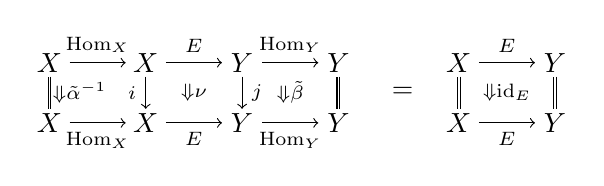
\begin{tikzpicture}[x=1.45em,y=1.45em]
  \node at (0,1.5)   {$X$};
  \node at (2.4,1.5) {$X$};
  \node at (4.8,1.5) {$Y$};
  \node at (7.2,1.5) {$Y$};
  \draw[->] (0.5,1.5) -- node[above]{$\scriptstyle\mathrm{Hom}_{X}$} (1.9,1.5);
  \draw[->] (2.9,1.5) -- node[above]{$\scriptstyle E$} (4.3,1.5);
  \draw[->] (5.3,1.5) -- node[above]{$\scriptstyle\mathrm{Hom}_{Y}$} (6.7,1.5);
  \draw[double,double distance=0.6pt] (0,1.15) -- (0,0.35);
  \node at (0.75,0.75) {$\scriptstyle\Downarrow\tilde{\alpha}^{-1}$};
  \draw[->] (2.4,1.15) -- node[left]{$\scriptstyle i$} (2.4,0.35);
  \node at (3.6,0.75) {$\scriptstyle\Downarrow\nu$};
  \draw[->] (4.8,1.15) -- node[right]{$\scriptstyle j$} (4.8,0.35);
  \node at (6.0,0.75) {$\scriptstyle\Downarrow\tilde{\beta}$};
  \draw[double,double distance=0.6pt] (7.2,1.15) -- (7.2,0.35);
  \node at (0,0)   {$X$};
  \node at (2.4,0) {$X$};
  \node at (4.8,0) {$Y$};
  \node at (7.2,0) {$Y$};
  \draw[->] (0.5,0) -- node[below]{$\scriptstyle\mathrm{Hom}_{X}$} (1.9,0);
  \draw[->] (2.9,0) -- node[below]{$\scriptstyle E$} (4.3,0);
  \draw[->] (5.3,0) -- node[below]{$\scriptstyle\mathrm{Hom}_{Y}$} (6.7,0);
  \node at (8.8,0.75) {$=$};
  \begin{scope}[shift={(10.2,0)}]
  \node at (0,1.5) {$X$};
  \node at (2.4,1.5) {$Y$};
  \draw[->] (0.5,1.5) -- node[above]{$\scriptstyle E$} (1.9,1.5);
  \draw[double,double distance=0.6pt] (0,1.15) -- (0,0.35);
  \node at (1.2,0.75) {$\scriptstyle\Downarrow\mathrm{id}_{E}$};
  \draw[double,double distance=0.6pt] (2.4,1.15) -- (2.4,0.35);
  \node at (0,0) {$X$};
  \node at (2.4,0) {$Y$};
  \draw[->] (0.5,0) -- node[below]{$\scriptstyle E$} (1.9,0);
  \end{scope}
\end{tikzpicture}
\end{center}
则 $\Mof{\C}\dot{I}_{C}\langle\nu\rangle$ 为单点集，否则为空；
\item 对 $i\colon \Mof{\C}A(X,X)$、$\alpha\colon \Mof{\C}I_{A}\langle i\rangle$、
$H\colon \Mof{\C}M(X,X)$ 与 $\theta\colon \Mof{\C}C_{0}\langle i,i,H\rangle$：
若零元复合\trCell
\begin{center}
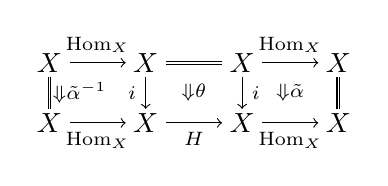
\begin{tikzpicture}[x=1.45em,y=1.45em]
  \node at (0,1.5)   {$X$};
  \node at (2.4,1.5) {$X$};
  \node at (4.8,1.5) {$X$};
  \node at (7.2,1.5) {$X$};
  \draw[->] (0.5,1.5) -- node[above]{$\scriptstyle\mathrm{Hom}_{X}$} (1.9,1.5);
  \draw[double,double distance=0.6pt] (2.9,1.5) -- (4.3,1.5);
  \draw[->] (5.3,1.5) -- node[above]{$\scriptstyle\mathrm{Hom}_{X}$} (6.7,1.5);
  \draw[double,double distance=0.6pt] (0,1.15) -- (0,0.35);
  \node at (0.75,0.75) {$\scriptstyle\Downarrow\tilde{\alpha}^{-1}$};
  \draw[->] (2.4,1.15) -- node[left]{$\scriptstyle i$} (2.4,0.35);
  \node at (3.6,0.75) {$\scriptstyle\Downarrow\theta$};
  \draw[->] (4.8,1.15) -- node[right]{$\scriptstyle i$} (4.8,0.35);
  \node at (6.0,0.75) {$\scriptstyle\Downarrow\tilde{\alpha}$};
  \draw[double,double distance=0.6pt] (7.2,1.15) -- (7.2,0.35);
  \node at (0,0)   {$X$};
  \node at (2.4,0) {$X$};
  \node at (4.8,0) {$X$};
  \node at (7.2,0) {$X$};
  \draw[->] (0.5,0) -- node[below]{$\scriptstyle\mathrm{Hom}_{X}$} (1.9,0);
  \draw[->] (2.9,0) -- node[below]{$\scriptstyle H$} (4.3,0);
  \draw[->] (5.3,0) -- node[below]{$\scriptstyle\mathrm{Hom}_{X}$} (6.7,0);
\end{tikzpicture}
\end{center}
是余笛卡尔的，则 $\Mof{\C}\dot{U}\langle i,\theta\rangle$ 为单点集，否则为空；
\item 对任何 $f\colon \Mof{\C}A(X,Y)$、$g\colon \Mof{\C}A(Y,Z)$ 与
$h\colon \Mof{\C}A(X,Z)$，$\Mof{\C}T\langle f,g,h\rangle$ 是竖直 2-范畴中可
逆\trCell{} $\gamma\colon gf\cong h$ 的集合；
\item 对任何 $n_{1}+\cdots+n_{k}=n$，给定诸\trCell
\begin{center}
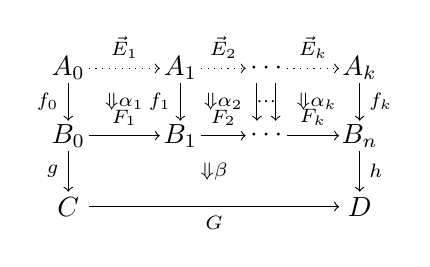
\begin{tikzpicture}[x=1.35em,y=1.35em]
  \node (A0) at (0,3.0)    {$A_{0}$};
  \node (A1) at (3.0,3.0)  {$A_{1}$};
  \node at (5.3,3.0)       {$\cdots$};
  \node (Ak) at (7.8,3.0)  {$A_{k}$};
  \draw[->,dotted] (0.55,3.0) -- node[above]{$\scriptstyle\vec{E}_{1}$} (2.45,3.0);
  \draw[->,dotted] (3.55,3.0) -- node[above]{$\scriptstyle\vec{E}_{2}$} (4.75,3.0);
  \draw[->,dotted] (5.85,3.0) -- node[above]{$\scriptstyle\vec{E}_{k}$} (7.25,3.0);
  \draw[->] (0,2.6) -- node[left]{$\scriptstyle f_{0}$} (0,1.6);
  \draw[->] (3.0,2.6) -- node[left]{$\scriptstyle f_{1}$} (3.0,1.6);
  \draw[->] (5.05,2.6) -- (5.05,1.6);
  \draw[->] (5.55,2.6) -- (5.55,1.6);
  \node at (5.3,2.1) {$\scriptstyle\cdots$};
  \draw[->] (7.8,2.6) -- node[right]{$\scriptstyle f_{k}$} (7.8,1.6);
  \node at (1.5,2.1)  {$\scriptstyle\Downarrow\alpha_{1}$};
  \node at (4.15,2.1) {$\scriptstyle\Downarrow\alpha_{2}$};
  \node at (6.65,2.1) {$\scriptstyle\Downarrow\alpha_{k}$};
  \node (B0) at (0,1.2)   {$B_{0}$};
  \node (B1) at (3.0,1.2) {$B_{1}$};
  \node at (5.3,1.2)      {$\cdots$};
  \node (Bn) at (7.8,1.2) {$B_{n}$};
  \draw[->] (0.55,1.2) -- node[above]{$\scriptstyle F_{1}$} (2.45,1.2);
  \draw[->] (3.55,1.2) -- node[above]{$\scriptstyle F_{2}$} (4.75,1.2);
  \draw[->] (5.85,1.2) -- node[above]{$\scriptstyle F_{k}$} (7.25,1.2);
  \draw[->] (0,0.8) -- node[left]{$\scriptstyle g$} (0,-0.3);
  \draw[->] (7.8,0.8) -- node[right]{$\scriptstyle h$} (7.8,-0.3);
  \node at (3.9,0.25) {$\scriptstyle\Downarrow\beta$};
  \node (C) at (0,-0.7)   {$C$};
  \node (D) at (7.8,-0.7) {$D$};
  \draw[->] (0.55,-0.7) -- node[below]{$\scriptstyle G$} (7.25,-0.7);
\end{tikzpicture}\\[1.2em]
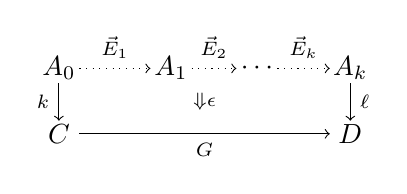
\begin{tikzpicture}[x=1.35em,y=1.35em]
  \node (A0) at (0,1.6)    {$A_{0}$};
  \node (A1) at (3.0,1.6)  {$A_{1}$};
  \node at (5.3,1.6)       {$\cdots$};
  \node (Ak) at (7.8,1.6)  {$A_{k}$};
  \draw[->,dotted] (0.55,1.6) -- node[above]{$\scriptstyle\vec{E}_{1}$} (2.45,1.6);
  \draw[->,dotted] (3.55,1.6) -- node[above]{$\scriptstyle\vec{E}_{2}$} (4.75,1.6);
  \draw[->,dotted] (5.85,1.6) -- node[above]{$\scriptstyle\vec{E}_{k}$} (7.25,1.6);
  \draw[->] (0,1.2) -- node[left]{$\scriptstyle k$} (0,0.2);
  \draw[->] (7.8,1.2) -- node[right]{$\scriptstyle\ell$} (7.8,0.2);
  \node at (3.9,0.7) {$\scriptstyle\Downarrow\epsilon$};
  \node (C) at (0,-0.15)   {$C$};
  \node (D) at (7.8,-0.15) {$D$};
  \draw[->] (0.55,-0.15) -- node[below]{$\scriptstyle G$} (7.25,-0.15);
\end{tikzpicture}
\end{center}
与任意一对同构 $\gamma\colon T\langle f_{0},g,k\rangle$ 与
$\delta\colon T\langle f_{k},h,\ell\rangle$：若 $\epsilon$ 等于复合
\begin{center}
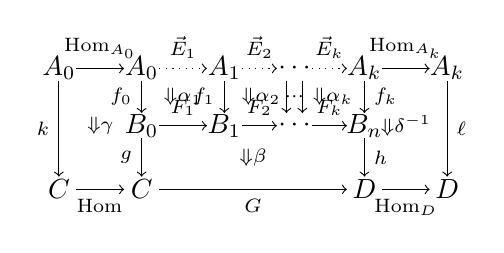
\begin{tikzpicture}[x=1.15em,y=1.15em]
  \node (A0a) at (0,3.0)    {$A_{0}$};
  \node (A0b) at (2.6,3.0)  {$A_{0}$};
  \node (A1)  at (5.2,3.0)  {$A_{1}$};
  \node at (7.4,3.0)        {$\cdots$};
  \node (Ak1) at (9.6,3.0)  {$A_{k}$};
  \node (Ak2) at (12.2,3.0) {$A_{k}$};
  \draw[->] (0.55,3.0) -- node[above]{$\scriptstyle\mathrm{Hom}_{A_{0}}$} (2.05,3.0);
  \draw[->,dotted] (3.15,3.0) -- node[above]{$\scriptstyle\vec{E}_{1}$} (4.65,3.0);
  \draw[->,dotted] (5.75,3.0) -- node[above]{$\scriptstyle\vec{E}_{2}$} (6.85,3.0);
  \draw[->,dotted] (7.95,3.0) -- node[above]{$\scriptstyle\vec{E}_{k}$} (9.05,3.0);
  \draw[->] (10.15,3.0) -- node[above]{$\scriptstyle\mathrm{Hom}_{A_{k}}$} (11.65,3.0);
  \draw[->] (0,2.6) -- node[left]{$\scriptstyle k$} (0,-0.4);
  \draw[->] (12.2,2.6) -- node[right]{$\scriptstyle\ell$} (12.2,-0.4);
  \draw[->] (2.6,2.6) -- node[left]{$\scriptstyle f_{0}$} (2.6,1.6);
  \draw[->] (5.2,2.6) -- node[left]{$\scriptstyle f_{1}$} (5.2,1.6);
  \draw[->] (7.15,2.6) -- (7.15,1.6);
  \draw[->] (7.65,2.6) -- (7.65,1.6);
  \node at (7.4,2.1) {$\scriptstyle\cdots$};
  \draw[->] (9.6,2.6) -- node[right]{$\scriptstyle f_{k}$} (9.6,1.6);
  \node at (3.9,2.1)  {$\scriptstyle\Downarrow\alpha_{1}$};
  \node at (6.35,2.1) {$\scriptstyle\Downarrow\alpha_{2}$};
  \node at (8.6,2.1)  {$\scriptstyle\Downarrow\alpha_{k}$};
  \node at (1.3,1.2)  {$\scriptstyle\Downarrow\gamma$};
  \node at (10.9,1.2) {$\scriptstyle\Downarrow\delta^{-1}$};
  \node (B0) at (2.6,1.2)  {$B_{0}$};
  \node (B1) at (5.2,1.2)  {$B_{1}$};
  \node at (7.4,1.2)       {$\cdots$};
  \node (Bn) at (9.6,1.2)  {$B_{n}$};
  \draw[->] (3.15,1.2) -- node[above]{$\scriptstyle F_{1}$} (4.65,1.2);
  \draw[->] (5.75,1.2) -- node[above]{$\scriptstyle F_{2}$} (6.85,1.2);
  \draw[->] (7.95,1.2) -- node[above]{$\scriptstyle F_{k}$} (9.05,1.2);
  \draw[->] (2.6,0.8) -- node[left]{$\scriptstyle g$} (2.6,-0.4);
  \draw[->] (9.6,0.8) -- node[right]{$\scriptstyle h$} (9.6,-0.4);
  \node at (6.1,0.2) {$\scriptstyle\Downarrow\beta$};
  \node (C0) at (0,-0.8)    {$C$};
  \node (C1) at (2.6,-0.8)  {$C$};
  \node (D1) at (9.6,-0.8)  {$D$};
  \node (D2) at (12.2,-0.8) {$D$};
  \draw[->] (0.55,-0.8) -- node[below]{$\scriptstyle\mathrm{Hom}_{\C}$} (2.05,-0.8);
  \draw[->] (3.15,-0.8) -- node[below]{$\scriptstyle G$} (9.05,-0.8);
  \draw[->] (10.15,-0.8) -- node[below]{$\scriptstyle\mathrm{Hom}_{\mathbb{D}}$} (11.65,-0.8);
\end{tikzpicture}
\end{center}
则集合 $\Mof{\C}\dot{T}_{n_{1},\ldots,n_{k}}\langle\alpha_{1},\ldots,\alpha_{k},\beta,\epsilon,\gamma,\delta\rangle$
为单点集，否则为空。
\end{itemize}
\end{definition}

我们记 $\Mof{\mathcal{K}}\colon \JVE\to\mathcal{S}et$ 为把%
\cref{def:ve-structure-of-virtual-equipment}的构造
施用于模的\trVirtualEquipment{} $\Mod(\mathcal{K})$ 而得的 $\JVE$-结构。

\begin{remark}\label{rem:natural-transformation-of-structures}
回顾：\trVirtualEquipment{}间的一个\trFunctor{} $F\colon\C\to\mathbb{D}$ 是
一个保持全部结构——包括单位\trCell{}与限制\trCell——的%
\trVirtualDoubleCategory{}间的映射。于是，施用 $F$ 便直接
给出了相应诸 $\JVE$-结构之间一个\trNaturalTransformation{}
$F\colon\Mof{\C}\to\Mof{\mathbb{D}}$ 的诸分量。依据%
\cref{prop:cosmological-functor-induces-ve-functor}，一个\trCosmologicalFunctor{}
$F\colon\mathcal{K}\to\mathcal{L}$ 诱导\trVirtualEquipment{}间的一个\trFunctor{}
$F\colon\Mod(\mathcal{K})\to\Mod(\mathcal{L})$，从而诱导 $\JVE$-结构之间的一
个\trNaturalTransformation{} $F\colon\Mof{\mathcal{K}}\to\Mof{\mathcal{L}}$。
\end{remark}

\begin{proposition}\label{prop:biequivalence-gives-ve-equivalence}
考虑由一个\trCosmologicalFunctor{} $F\colon\mathcal{K}\to\mathcal{L}$ 相连的
一对\trInfinityCosmos。
\begin{enumerate}[label=(\roman*)]
\item 若 $F\colon\mathcal{K}\to\mathcal{L}$ 是一个\trCosmologicalBiequivalence，
则在相应的诸 $\JVE$-结构之间存在一对逐纤维满射：
\begin{center}
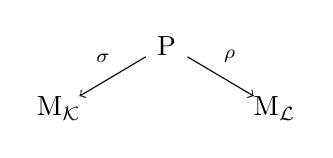
\begin{tikzpicture}[x=1.5em,y=1.5em]
  \node (P) at (0,1.5)  {$\mathrm{P}$};
  \node (K) at (-2.6,0) {$\Mof{\mathcal{K}}$};
  \node (L) at (2.6,0)  {$\Mof{\mathcal{L}}$};
  \draw[->] (-0.5,1.25) -- node[above left,pos=0.4]{$\scriptstyle\sigma$} (-2.1,0.3);
  \draw[->] (0.5,1.25) -- node[above right,pos=0.4]{$\scriptstyle\rho$} (2.1,0.3);
\end{tikzpicture}
\end{center}
\item 此外，若 $\JVE$-结构之间的受诱导映射保持一个上下文 $\Gamma$
的给定解释
\begin{center}
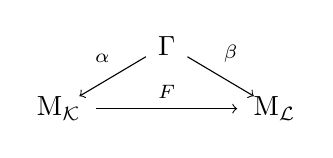
\begin{tikzpicture}[x=1.5em,y=1.5em]
  \node (G) at (0,1.5)  {$\Gamma$};
  \node (K) at (-2.6,0) {$\Mof{\mathcal{K}}$};
  \node (L) at (2.6,0)  {$\Mof{\mathcal{L}}$};
  \draw[->] (-0.5,1.25) -- node[above left,pos=0.4]{$\scriptstyle\alpha$} (-2.1,0.3);
  \draw[->] (0.5,1.25) -- node[above right,pos=0.4]{$\scriptstyle\beta$} (2.1,0.3);
  \draw[->] (-1.7,0) -- node[above]{$\scriptstyle F$} (1.7,0);
\end{tikzpicture}
\end{center}
则 (i) 中构造的诸逐纤维满射给出上下文 $\Gamma$ 中的一个 $\JVE$-等价：
\begin{center}
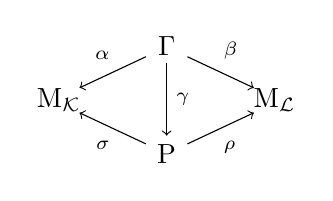
\begin{tikzpicture}[x=1.5em,y=1.5em]
  \node (G) at (0,2.6)  {$\Gamma$};
  \node (K) at (-2.6,1.3) {$\Mof{\mathcal{K}}$};
  \node (L) at (2.6,1.3)  {$\Mof{\mathcal{L}}$};
  \node (P) at (0,0)    {$\mathrm{P}$};
  \draw[->] (-0.5,2.35) -- node[above left,pos=0.4]{$\scriptstyle\alpha$} (-2.1,1.6);
  \draw[->] (0.5,2.35) -- node[above right,pos=0.4]{$\scriptstyle\beta$} (2.1,1.6);
  \draw[->] (0,2.2) -- node[right]{$\scriptstyle\gamma$} (0,0.45);
  \draw[->] (-0.5,0.25) -- node[below left,pos=0.4]{$\scriptstyle\sigma$} (-2.1,1.0);
  \draw[->] (0.5,0.25) -- node[below right,pos=0.4]{$\scriptstyle\rho$} (2.1,1.0);
\end{tikzpicture}
\end{center}
\end{enumerate}
\end{proposition}

\begin{proof}
我们采用与\cref{exa:jcat-equivalence-iso-comma}和\cref{exa:pseudo-comma-2-category}中相同的策略，构造一个结构，称之为与%
\trVirtualEquipment{}间的\trFunctor{}
$F\colon\Mod(\mathcal{K})\to\Mod(\mathcal{L})$ 相关联的%
\emph{伪逗号\trVirtualEquipment}（pseudo-comma virtual equipment）$\mathbb{P}$。\footnote{%
伪逗号\trVirtualEquipment{}对\trVirtualEquipment{}之间的任何\trFunctor（或更
一般地，\trFunctor{}的%
\trCospan）都可用完全相同的方式定义；但在记号得以简化之处，我们亦将此种说法
用于\trInfinityCosmos{}中的结构及其\trHomotopyTwoCategory。}
$\JVE$-结构 $\mathrm{P}$ 随之定义为 $\Mof{\mathbb{P}}$，而 $\sigma$ 与 $\rho$
则是显然的投射。然后我们论证：在 $F$ 是\trVirtualEquipment{}间的一个%
\trBiequivalence{}这一假设下，这两个映射是逐纤维满的。

与 $F\colon\Mod(\mathcal{K})\to\Mod(\mathcal{L})$ 相关联的\textbf{伪逗号%
\trVirtualEquipment} $\mathbb{P}$ 拥有：
\begin{itemize}
\item 对象由三元组 $(A\in\mathcal{K},\,A'\in\mathcal{L},\,a\colon FA\Rightarrow A'\in\mathcal{L})$
给出，其中 $a$ 是一个\trEquivalence；
\item 竖直箭头 $(A,A',a)\to(B,B',b)$ 由如下形状的三元组给出
\[
\left(\;
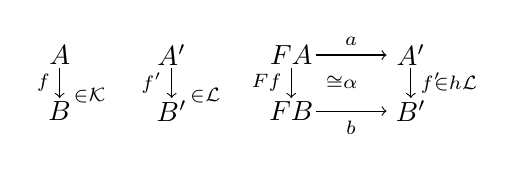
\begin{tikzpicture}[x=1.35em,y=1.35em]
  \node at (0,1.5)    {$A$};
  \node at (3.0,1.5)  {$A'$};
  \node at (6.2,1.5)  {$FA$};
  \node at (9.4,1.5)  {$A'$};
  \draw[->] (6.85,1.5) -- node[above]{$\scriptstyle a$} (8.75,1.5);
  \draw[->] (0,1.15) -- node[left]{$\scriptstyle f$} (0,0.35);
  \node at (0.8,0.4) {$\scriptstyle\in\mathcal{K}$};
  \draw[->] (3.0,1.15) -- node[left]{$\scriptstyle f'$} (3.0,0.35);
  \node at (3.9,0.4) {$\scriptstyle\in\mathcal{L}$};
  \draw[->] (6.2,1.15) -- node[left]{$\scriptstyle Ff$} (6.2,0.35);
  \node at (7.55,0.75) {$\scriptstyle\cong\alpha$};
  \draw[->] (9.4,1.15) -- node[right]{$\scriptstyle f'$} (9.4,0.35);
  \node at (10.6,0.75) {$\scriptstyle\in\mathfrak{h}\mathcal{L}$};
  \node at (0,0)    {$B$};
  \node at (3.0,0)  {$B'$};
  \node at (6.2,0)  {$FB$};
  \node at (9.4,0)  {$B'$};
  \draw[->] (6.85,0) -- node[below]{$\scriptstyle b$} (8.75,0);
\end{tikzpicture}
\;\right)
\]
\item 模 $(A,A',a)\longmapsto(B,B',b)$ 由如下形状的三元组给出
\[
\left(\;
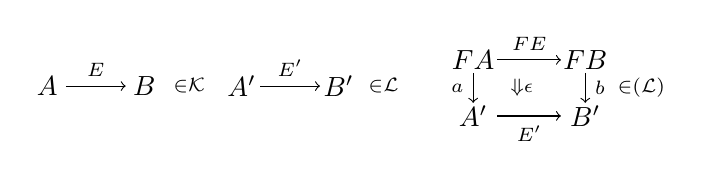
\begin{tikzpicture}[x=1.35em,y=1.35em]
  \node at (0,1.4)   {$A$};
  \node at (2.6,1.4) {$B$};
  \draw[->] (0.5,1.4) -- node[above]{$\scriptstyle E$} (2.1,1.4);
  \node at (3.8,1.4) {$\scriptstyle\in\mathcal{K}$};
  \node at (5.2,1.4)  {$A'$};
  \node at (7.8,1.4)  {$B'$};
  \draw[->] (5.7,1.4) -- node[above]{$\scriptstyle E'$} (7.3,1.4);
  \node at (9.0,1.4) {$\scriptstyle\in\mathcal{L}$};
  \node at (11.4,2.1) {$FA$};
  \node at (14.4,2.1) {$FB$};
  \draw[->] (12.05,2.1) -- node[above]{$\scriptstyle FE$} (13.75,2.1);
  \draw[->] (11.4,1.75) -- node[left]{$\scriptstyle a$} (11.4,0.95);
  \node at (12.7,1.35) {$\scriptstyle\Downarrow\epsilon$};
  \draw[->] (14.4,1.75) -- node[right]{$\scriptstyle b$} (14.4,0.95);
  \node at (11.4,0.6)  {$A'$};
  \node at (14.4,0.6)  {$B'$};
  \draw[->] (12.05,0.6) -- node[below]{$\scriptstyle E'$} (13.75,0.6);
  \node at (15.9,1.35) {$\scriptstyle\in\Mod(\mathcal{L})$};
\end{tikzpicture}
\;\right)
\]
其中 $\epsilon$ 是一支\trCartesian\trCell；
\item $n$ 元\trCell{}由一对 $n$ 元\trCell——$\mathcal{K}$ 中的 $\mu$ 与
$\mathcal{L}$ 中的 $\nu$——给出，使得由其边界数据形成的复合\trCell{}相等：
\begin{center}
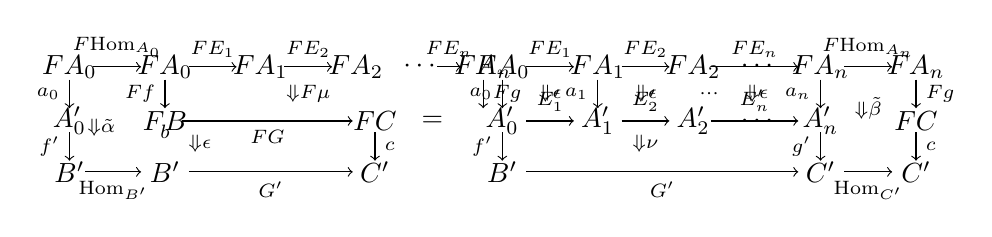
\begin{tikzpicture}[x=1.15em,y=1.15em]
  \node at (0,2.6)     {$FA_{0}$};
  \node at (3.0,2.6)   {$FA_{0}$};
  \node at (6.0,2.6)   {$FA_{1}$};
  \node at (9.0,2.6)   {$FA_{2}$};
  \node at (11.0,2.6)  {$\cdots$};
  \node at (13.0,2.6)  {$FA_{n}$};
  \draw[->] (0.75,2.6) -- node[above]{$\scriptstyle F\mathrm{Hom}_{A_{0}}$} (2.25,2.6);
  \draw[->] (3.75,2.6) -- node[above]{$\scriptstyle FE_{1}$} (5.25,2.6);
  \draw[->] (6.75,2.6) -- node[above]{$\scriptstyle FE_{2}$} (8.25,2.6);
  \draw[->] (11.55,2.6) -- node[above]{$\scriptstyle FE_{n}$} (12.3,2.6);
  \draw[->] (0,2.2) -- node[left]{$\scriptstyle a_{0}$} (0,1.3);
  \draw[->] (3.0,2.2) -- node[left]{$\scriptstyle Ff$} (3.0,1.3);
  \node at (7.5,1.75) {$\scriptstyle\Downarrow F\mu$};
  \draw[->] (13.0,2.2) -- node[right]{$\scriptstyle Fg$} (13.0,1.3);
  \node at (0,0.9)  {$A'_{0}$};
  \node at (3.0,0.9){$FB$};
  \node at (9.6,0.9){$FC$};
  \draw[->] (0,0.55) -- node[left]{$\scriptstyle f'$} (0,-0.35);
  \node at (1.0,0.7) {$\scriptstyle\Downarrow\tilde{\alpha}$};
  \node at (3.0,0.55) {$\scriptstyle b$};
  \draw[->] (3.55,0.9) -- node[below]{$\scriptstyle FG$} (8.9,0.9);
  \draw[->] (9.6,0.55) -- node[right]{$\scriptstyle c$} (9.6,-0.35);
  \node at (4.1,0.2) {$\scriptstyle\Downarrow\epsilon$};
  \node at (0,-0.7)  {$B'$};
  \node at (3.0,-0.7){$B'$};
  \node at (9.6,-0.7){$C'$};
  \draw[->] (0.5,-0.7) -- node[below]{$\scriptstyle\mathrm{Hom}_{B'}$} (2.25,-0.7);
  \draw[->] (3.75,-0.7) -- node[below]{$\scriptstyle G'$} (8.9,-0.7);
  \node at (11.4,0.9) {$=$};
  \begin{scope}[shift={(13.6,0)}]
  \node at (0,2.6)     {$FA_{0}$};
  \node at (3.0,2.6)   {$FA_{1}$};
  \node at (6.0,2.6)   {$FA_{2}$};
  \node at (8.0,2.6)   {$\cdots$};
  \node at (10.0,2.6)  {$FA_{n}$};
  \node at (13.0,2.6)  {$FA_{n}$};
  \draw[->] (0.75,2.6) -- node[above]{$\scriptstyle FE_{1}$} (2.25,2.6);
  \draw[->] (3.75,2.6) -- node[above]{$\scriptstyle FE_{2}$} (5.25,2.6);
  \draw[->] (6.55,2.6) -- node[above]{$\scriptstyle FE_{n}$} (9.3,2.6);
  \draw[->] (10.75,2.6) -- node[above]{$\scriptstyle F\mathrm{Hom}_{A_{n}}$} (12.25,2.6);
  \draw[->] (0,2.2) -- node[left]{$\scriptstyle a_{0}$} (0,1.3);
  \node at (1.5,1.75) {$\scriptstyle\Downarrow\epsilon$};
  \draw[->] (3.0,2.2) -- node[left]{$\scriptstyle a_{1}$} (3.0,1.3);
  \node at (4.5,1.75) {$\scriptstyle\Downarrow\epsilon$};
  \node at (6.5,1.75) {$\scriptstyle\cdots$};
  \node at (8.0,1.75) {$\scriptstyle\Downarrow\epsilon$};
  \draw[->] (10.0,2.2) -- node[left]{$\scriptstyle a_{n}$} (10.0,1.3);
  \draw[->] (13.0,2.2) -- node[right]{$\scriptstyle Fg$} (13.0,1.3);
  \node at (0,0.9)   {$A'_{0}$};
  \node at (3.0,0.9) {$A'_{1}$};
  \node at (6.0,0.9) {$A'_{2}$};
  \node at (8.0,0.9) {$\cdots$};
  \node at (10.0,0.9){$A'_{n}$};
  \node at (13.0,0.9){$FC$};
  \draw[->] (0.75,0.9) -- node[above]{$\scriptstyle E'_{1}$} (2.25,0.9);
  \draw[->] (3.75,0.9) -- node[above]{$\scriptstyle E'_{2}$} (5.25,0.9);
  \draw[->] (6.55,0.9) -- node[above]{$\scriptstyle E'_{n}$} (9.3,0.9);
  \node at (11.5,1.3) {$\scriptstyle\Downarrow\tilde{\beta}$};
  \draw[->] (0,0.55) -- node[left]{$\scriptstyle f'$} (0,-0.35);
  \node at (4.5,0.2) {$\scriptstyle\Downarrow\nu$};
  \draw[->] (10.0,0.55) -- node[left]{$\scriptstyle g'$} (10.0,-0.35);
  \draw[->] (13.0,0.55) -- node[right]{$\scriptstyle c$} (13.0,-0.35);
  \node at (0,-0.7)  {$B'$};
  \node at (10.0,-0.7){$C'$};
  \node at (13.0,-0.7){$C'$};
  \draw[->] (0.75,-0.7) -- node[below]{$\scriptstyle G'$} (9.3,-0.7);
  \draw[->] (10.75,-0.7) -- node[below]{$\scriptstyle\mathrm{Hom}_{C'}$} (12.25,-0.7);
  \end{scope}
\end{tikzpicture}
\end{center}
\end{itemize}

我们来论证 $\mathbb{P}$ 是一个\trVirtualDoubleCategory。注意其对象与竖直箭头
构成一个\trCategory：事实上，它正是\cref{exa:pseudo-comma-2-category}中\trTwoFunctor
$F\colon\mathfrak{h}\mathcal{K}\to\mathfrak{h}\mathcal{L}$ 的伪逗号 2-范畴的
底 1-范畴。每个模 $(E,E',\epsilon)\colon(A,A',a)\longmapsto(B,B',b)$ 都拥有
一支恒同\trCell，其分量为 $\mathcal{K}$ 中的恒同\trCell{} $\mathrm{id}_{E}$ 与
$\mathcal{L}$ 中的恒同\trCell{} $\mathrm{id}_{E'}$。诸\trCell{}的复合承袭自
$\Mod(\mathcal{K})$ 与 $\Mod(\mathcal{L})$，不过所需的、以这种方式定义的复合%
\trCell{}之间的粘贴等式，我们留给读者画一张非常大的图来验证。这使得
$\mathbb{P}$ 成为一个\trVirtualDoubleCategory。

事实上，$\mathbb{P}$ 是一个\trVirtualEquipment。每个对象 $(A,A',a)$ 容许
形如 $(\mathrm{Hom}_{A},\mathrm{Hom}_{A'},\mathrm{Hom}_{a})$ 的一个单位模，
并配备一支零元%
\trCocartesian\trCell
\begin{center}
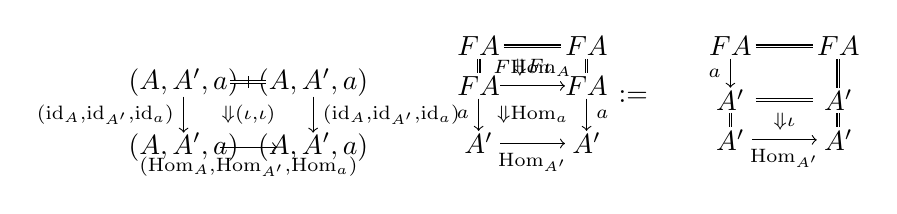
\begin{tikzpicture}[x=1.3em,y=1.3em]
  \node at (0,1.9)   {$(A,A',a)$};
  \node at (3.6,1.9) {$(A,A',a)$};
  \draw[double,double distance=0.6pt] (1.3,1.9) -- (2.3,1.9);
  \draw (1.8,2.07) -- (1.8,1.73);
  \draw[->] (0,1.5) -- node[left]{$\scriptstyle(\mathrm{id}_{A},\mathrm{id}_{A'},\mathrm{id}_{a})$} (0,0.5);
  \node at (1.8,1.0) {$\scriptstyle\Downarrow(\iota,\iota)$};
  \draw[->] (3.6,1.5) -- node[right]{$\scriptstyle(\mathrm{id}_{A},\mathrm{id}_{A'},\mathrm{id}_{a})$} (3.6,0.5);
  \node at (0,0.1)   {$(A,A',a)$};
  \node at (3.6,0.1) {$(A,A',a)$};
  \draw[->] (1.0,0.1) -- node[below]{$\scriptstyle(\mathrm{Hom}_{A},\mathrm{Hom}_{A'},\mathrm{Hom}_{a})$} (2.6,0.1);
  \node at (5.3,1.0) {$\scriptstyle\leftrightsquigarrow$};
  \begin{scope}[shift={(6.8,0)}]
  \node at (1.4,2.9) {$FA$};
  \node at (4.4,2.9) {$FA$};
  \draw[double,double distance=0.6pt] (2.1,2.9) -- (3.7,2.9);
  \draw[double,double distance=0.6pt] (1.4,2.55) -- (1.4,2.15);
  \draw[double,double distance=0.6pt] (4.4,2.55) -- (4.4,2.15);
  \node at (2.9,2.3) {$\scriptstyle\Downarrow F\iota$};
  \node at (1.4,1.8) {$FA$};
  \node at (4.4,1.8) {$FA$};
  \draw[->] (2.0,1.8) -- node[above]{$\scriptstyle F\mathrm{Hom}_{A}$} (3.8,1.8);
  \draw[->] (1.4,1.45) -- node[left]{$\scriptstyle a$} (1.4,0.55);
  \node at (2.9,1.0) {$\scriptstyle\Downarrow\mathrm{Hom}_{a}$};
  \draw[->] (4.4,1.45) -- node[right]{$\scriptstyle a$} (4.4,0.55);
  \node at (1.4,0.2)  {$A'$};
  \node at (4.4,0.2)  {$A'$};
  \draw[->] (2.0,0.2) -- node[below]{$\scriptstyle\mathrm{Hom}_{A'}$} (3.8,0.2);
  \end{scope}
  \node at (12.5,1.5) {$:=$};
  \begin{scope}[shift={(13.8,0)}]
  \node at (1.4,2.9) {$FA$};
  \node at (4.4,2.9) {$FA$};
  \draw[double,double distance=0.6pt] (2.1,2.9) -- (3.7,2.9);
  \draw[->] (1.4,2.55) -- node[left]{$\scriptstyle a$} (1.4,1.75);
  \draw[double,double distance=0.6pt] (4.4,2.55) -- (4.4,1.75);
  \node at (1.4,1.4) {$A'$};
  \node at (4.4,1.4) {$A'$};
  \draw[double,double distance=0.6pt] (2.1,1.4) -- (3.7,1.4);
  \draw[double,double distance=0.6pt] (1.4,1.05) -- (1.4,0.65);
  \draw[double,double distance=0.6pt] (4.4,1.05) -- (4.4,0.65);
  \node at (2.9,0.8) {$\scriptstyle\Downarrow\iota$};
  \node at (1.4,0.3)  {$A'$};
  \node at (4.4,0.3)  {$A'$};
  \draw[->] (2.0,0.3) -- node[below]{$\scriptstyle\mathrm{Hom}_{A'}$} (3.8,0.3);
  \end{scope}
\end{tikzpicture}
\end{center}
其两条竖直箭头均取为恒同 $(\mathrm{id}_{A},\mathrm{id}_{A'},\mathrm{id}_{a})$，
而其在 $\mathcal{K}$ 与 $\mathcal{L}$ 中的分量\trCell{}分别是 $A$ 与 $A'$ 的
单位\trCell。由于 $F$ 保持\trCocartesian\trCell，$F\iota$ 的%
\trUniversalProperty{}可用来定义一支满足所需粘贴等式的\trCell{}
$\mathrm{Hom}_{a}$（与第 8 章中的%
\cref{def:unary-unit-cell}相比较）。由于两个分量都定义\trCocartesian\trCell，
这支\trCell{}在 $\mathbb{P}$ 中是余笛卡尔的。

最后，任何由两条竖直箭头与一支水平\trModule{}组成的\trDiagram
\begin{center}
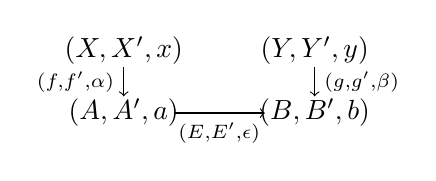
\begin{tikzpicture}[x=1.5em,y=1.5em]
  \node at (0,1.5)   {$(X,X',x)$};
  \node at (4.6,1.5) {$(Y,Y',y)$};
  \draw[->] (0,1.1) -- node[left]{$\scriptstyle(f,f',\alpha)$} (0,0.4);
  \draw[->] (4.6,1.1) -- node[right]{$\scriptstyle(g,g',\beta)$} (4.6,0.4);
  \node at (0,0)   {$(A,A',a)$};
  \node at (4.6,0) {$(B,B',b)$};
  \draw[->] (1.2,0) -- node[below]{$\scriptstyle(E,E',\epsilon)$} (3.4,0);
\end{tikzpicture}
\end{center}
都可以补全为一支一元\trCartesian\trCell
\begin{center}
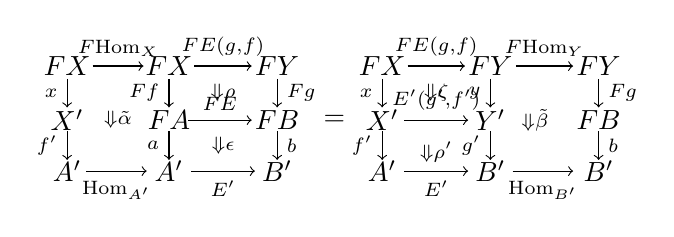
\begin{tikzpicture}[x=1.15em,y=1.15em]
  \node at (0,2.6)    {$FX$};
  \node at (3.2,2.6)  {$FX$};
  \node at (6.6,2.6)  {$FY$};
  \draw[->] (0.8,2.6) -- node[above]{$\scriptstyle F\mathrm{Hom}_{X}$} (2.4,2.6);
  \draw[->] (4.0,2.6) -- node[above]{$\scriptstyle FE(g,f)$} (5.8,2.6);
  \draw[->] (0,2.2) -- node[left]{$\scriptstyle x$} (0,1.3);
  \draw[->] (3.2,2.2) -- node[left]{$\scriptstyle Ff$} (3.2,1.3);
  \node at (4.9,1.75) {$\scriptstyle\Downarrow\rho$};
  \draw[->] (6.6,2.2) -- node[right]{$\scriptstyle Fg$} (6.6,1.3);
  \node at (0,0.9)  {$X'$};
  \node at (3.2,0.9){$FA$};
  \node at (6.6,0.9){$FB$};
  \node at (1.6,0.9) {$\scriptstyle\Downarrow\tilde{\alpha}$};
  \draw[->] (3.8,0.9) -- node[above]{$\scriptstyle FE$} (5.8,0.9);
  \draw[->] (0,0.55) -- node[left]{$\scriptstyle f'$} (0,-0.35);
  \draw[->] (3.2,0.55) -- node[left]{$\scriptstyle a$} (3.2,-0.35);
  \node at (4.9,0.1) {$\scriptstyle\Downarrow\epsilon$};
  \draw[->] (6.6,0.55) -- node[right]{$\scriptstyle b$} (6.6,-0.35);
  \node at (0,-0.7)  {$A'$};
  \node at (3.2,-0.7){$A'$};
  \node at (6.6,-0.7){$B'$};
  \draw[->] (0.6,-0.7) -- node[below]{$\scriptstyle\mathrm{Hom}_{A'}$} (2.5,-0.7);
  \draw[->] (3.9,-0.7) -- node[below]{$\scriptstyle E'$} (5.9,-0.7);
  \node at (8.4,0.9) {$=$};
  \begin{scope}[shift={(9.9,0)}]
  \node at (0,2.6)   {$FX$};
  \node at (3.4,2.6) {$FY$};
  \node at (6.8,2.6) {$FY$};
  \draw[->] (0.8,2.6) -- node[above]{$\scriptstyle FE(g,f)$} (2.6,2.6);
  \draw[->] (4.2,2.6) -- node[above]{$\scriptstyle F\mathrm{Hom}_{Y}$} (6.0,2.6);
  \draw[->] (0,2.2) -- node[left]{$\scriptstyle x$} (0,1.3);
  \node at (1.7,1.75) {$\scriptstyle\Downarrow\zeta$};
  \draw[->] (3.4,2.2) -- node[left]{$\scriptstyle y$} (3.4,1.3);
  \draw[->] (6.8,2.2) -- node[right]{$\scriptstyle Fg$} (6.8,1.3);
  \node at (0,0.9)   {$X'$};
  \node at (3.4,0.9) {$Y'$};
  \node at (6.8,0.9) {$FB$};
  \draw[->] (0.7,0.9) -- node[above]{$\scriptstyle E'(g',f')$} (2.7,0.9);
  \node at (4.8,0.9) {$\scriptstyle\Downarrow\tilde{\beta}$};
  \draw[->] (0,0.55) -- node[left]{$\scriptstyle f'$} (0,-0.35);
  \node at (1.7,-0.1) {$\scriptstyle\Downarrow\rho'$};
  \draw[->] (3.4,0.55) -- node[left]{$\scriptstyle g'$} (3.4,-0.35);
  \draw[->] (6.8,0.55) -- node[right]{$\scriptstyle b$} (6.8,-0.35);
  \node at (0,-0.7)  {$A'$};
  \node at (3.4,-0.7){$B'$};
  \node at (6.8,-0.7){$B'$};
  \draw[->] (0.7,-0.7) -- node[below]{$\scriptstyle E'$} (2.7,-0.7);
  \draw[->] (4.1,-0.7) -- node[below]{$\scriptstyle\mathrm{Hom}_{B'}$} (6.0,-0.7);
  \end{scope}
\end{tikzpicture}
\end{center}
其中 $\rho$ 与 $\rho'$ 分别是 $\mathcal{K}$ 与 $\mathcal{L}$ 中的限制\trCell，
而\trCell{} $\zeta$ 则定义为把下面的左手\trPastingDiagram{}穿过\trCartesian\trCell{} $\rho'$
作分解所得者：
\begin{center}
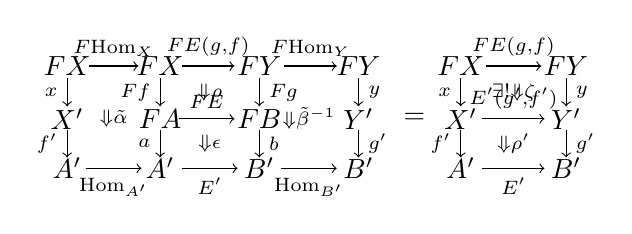
\begin{tikzpicture}[x=1.12em,y=1.12em]
  \node at (0,2.6)    {$FX$};
  \node at (3.0,2.6)  {$FX$};
  \node at (6.2,2.6)  {$FY$};
  \node at (9.4,2.6)  {$FY$};
  \draw[->] (0.7,2.6) -- node[above]{$\scriptstyle F\mathrm{Hom}_{X}$} (2.3,2.6);
  \draw[->] (3.7,2.6) -- node[above]{$\scriptstyle FE(g,f)$} (5.4,2.6);
  \draw[->] (7.0,2.6) -- node[above]{$\scriptstyle F\mathrm{Hom}_{Y}$} (8.7,2.6);
  \draw[->] (0,2.2) -- node[left]{$\scriptstyle x$} (0,1.3);
  \draw[->] (3.0,2.2) -- node[left]{$\scriptstyle Ff$} (3.0,1.3);
  \node at (4.6,1.75) {$\scriptstyle\Downarrow\rho$};
  \draw[->] (6.2,2.2) -- node[right]{$\scriptstyle Fg$} (6.2,1.3);
  \draw[->] (9.4,2.2) -- node[right]{$\scriptstyle y$} (9.4,1.3);
  \node at (0,0.9)  {$X'$};
  \node at (3.0,0.9){$FA$};
  \node at (6.2,0.9){$FB$};
  \node at (9.4,0.9){$Y'$};
  \node at (1.5,0.9) {$\scriptstyle\Downarrow\tilde{\alpha}$};
  \draw[->] (3.6,0.9) -- node[above]{$\scriptstyle FE$} (5.4,0.9);
  \node at (7.8,0.9) {$\scriptstyle\Downarrow\tilde{\beta}^{-1}$};
  \draw[->] (0,0.55) -- node[left]{$\scriptstyle f'$} (0,-0.35);
  \draw[->] (3.0,0.55) -- node[left]{$\scriptstyle a$} (3.0,-0.35);
  \node at (4.6,0.1) {$\scriptstyle\Downarrow\epsilon$};
  \draw[->] (6.2,0.55) -- node[right]{$\scriptstyle b$} (6.2,-0.35);
  \draw[->] (9.4,0.55) -- node[right]{$\scriptstyle g'$} (9.4,-0.35);
  \node at (0,-0.7)  {$A'$};
  \node at (3.0,-0.7){$A'$};
  \node at (6.2,-0.7){$B'$};
  \node at (9.4,-0.7){$B'$};
  \draw[->] (0.6,-0.7) -- node[below]{$\scriptstyle\mathrm{Hom}_{A'}$} (2.4,-0.7);
  \draw[->] (3.7,-0.7) -- node[below]{$\scriptstyle E'$} (5.5,-0.7);
  \draw[->] (6.9,-0.7) -- node[below]{$\scriptstyle\mathrm{Hom}_{B'}$} (8.7,-0.7);
  \node at (11.2,0.9) {$=$};
  \begin{scope}[shift={(12.7,0)}]
  \node at (0,2.6)   {$FX$};
  \node at (3.4,2.6) {$FY$};
  \draw[->] (0.8,2.6) -- node[above]{$\scriptstyle FE(g,f)$} (2.6,2.6);
  \draw[->] (0,2.2) -- node[left]{$\scriptstyle x$} (0,1.3);
  \node at (1.7,1.75) {$\scriptstyle\exists!\Downarrow\zeta$};
  \draw[->] (3.4,2.2) -- node[right]{$\scriptstyle y$} (3.4,1.3);
  \node at (0,0.9)   {$X'$};
  \node at (3.4,0.9) {$Y'$};
  \draw[->] (0.7,0.9) -- node[above]{$\scriptstyle E'(g',f')$} (2.7,0.9);
  \draw[->] (0,0.55) -- node[left]{$\scriptstyle f'$} (0,-0.35);
  \node at (1.7,0.1) {$\scriptstyle\Downarrow\rho'$};
  \draw[->] (3.4,0.55) -- node[right]{$\scriptstyle g'$} (3.4,-0.35);
  \node at (0,-0.7)  {$A'$};
  \node at (3.4,-0.7){$B'$};
  \draw[->] (0.7,-0.7) -- node[below]{$\scriptstyle E'$} (2.7,-0.7);
  \end{scope}
\end{tikzpicture}
\end{center}
由于 $\epsilon$、$F\rho$ 与 $\rho'$ 都是 $\mathcal{L}$ 中的\trCartesian\trCell，
$\zeta$ 也是一支\trCartesian\trCell，这就使
$(E(g,f),\,E'(g',f'),\,\zeta)$ 成为 $\mathbb{P}$ 中的一个\trModule。这使得
虚拟双范畴 $\mathbb{P}$ 成为一个虚拟装备，且到 $\Mod(\mathcal{K})$ 与
$\Mod(\mathcal{L})$ 的显然遗忘函子定义虚拟装备间的\trFunctor。

依据\cref{rem:natural-transformation-of-structures}，我们得到一个由 $\JVE$-结
构与\trNaturalTransformation{}组成的图表
\begin{center}
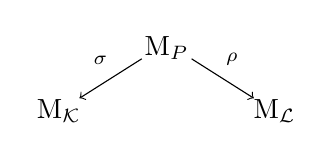
\begin{tikzpicture}[x=1.5em,y=1.5em]
  \node (P) at (0,1.5)  {$\Mof{\mathbb{P}}$};
  \node (K) at (-2.6,0) {$\Mof{\mathcal{K}}$};
  \node (L) at (2.6,0)  {$\Mof{\mathcal{L}}$};
  \draw[->] (-0.6,1.25) -- node[above left,pos=0.4]{$\scriptstyle\sigma$} (-2.1,0.3);
  \draw[->] (0.6,1.25) -- node[above right,pos=0.4]{$\scriptstyle\rho$} (2.1,0.3);
\end{tikzpicture}
\end{center}
最后，当 $F\colon\Mod(\mathcal{K})\to\Mod(\mathcal{L})$ 是\trVirtualEquipment{}%
间的一个%
\trBiequivalence——即满足\cref{thm:biequivalence-of-virtual-equipments}所列
诸性质——时，\trForgetfulFunctor
\begin{equation*}
\Mod(\mathcal{K}) \;\longleftarrow\; \mathbb{P} \;\longrightarrow\; \Mod(\mathcal{L})
\end{equation*}
在对象上满、在竖直箭头上满、在水平\trModule{}上满、在\trCell{}上%
\trFullyFaithful，并且反射单
位\trCell{}与限制\trCell。由此可知，映射 $\sigma$ 与 $\rho$ 是逐纤维满的。

最后，若 $F\colon\Mof{\mathcal{K}}\to\Mof{\mathcal{L}}$ 严格保持一个上下文
$\Gamma$ 在 $\Mod(\mathcal{K})$ 与 $\Mod(\mathcal{L})$ 中的诸解释，我们断言：
可以沿 $\sigma$ 与 $\rho$ 同时把这些解释提升为一个解释
$\gamma\colon\Gamma\to\mathbb{P}$。这可以在 $\JVE$-结构 $\Gamma$ 中容易地归
纳验证。对一个变量（variable）$x\colon O$，若 $\alpha(x)=A$ 且
$\beta(x)=FA$，则定义 $\gamma(x)\coloneqq(A,FA,\mathrm{id}_{FA})$。$\gamma$
在更高次的变量处的定义与之类似，缺失的数据取为 $\mathcal{L}$ 中适当的恒同。
\end{proof}

将这几项结果合在一起，我们便得到所期望的推论：

\begin{corollary}[模型无关∞-范畴论的语言]\label{cor:language-for-model-independence}
\trVirtualEquipment{}的语言中的公式在\trInfinityCosmos{}的\trBiequivalence{}之下不变。
\end{corollary}

\begin{proof}
考虑\trVirtualEquipment{}的语言中的一个公式 $\phi$，其自由变量（free variables）的解释相
容地定义，意即存在一个交换图
\begin{center}
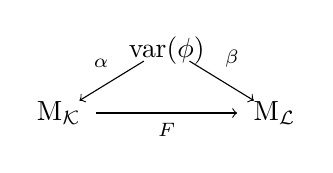
\begin{tikzpicture}[x=1.5em,y=1.5em]
  \node (V) at (0,1.5)  {$\mathrm{var}(\phi)$};
  \node (K) at (-2.6,0) {$\Mof{\mathcal{K}}$};
  \node (L) at (2.6,0)  {$\Mof{\mathcal{L}}$};
  \draw[->] (-0.55,1.25) -- node[above left,pos=0.4]{$\scriptstyle\alpha$} (-2.1,0.3);
  \draw[->] (0.55,1.25) -- node[above right,pos=0.4]{$\scriptstyle\beta$} (2.1,0.3);
  \draw[->] (-1.7,0) -- node[below]{$\scriptstyle F$} (1.7,0);
\end{tikzpicture}
\end{center}
它由\trCosmologicalBiequivalence{} $F\colon\mathcal{K}\simeq\mathcal{L}$ 与
\cref{def:ve-structure-of-virtual-equipment}所规定的诸 $\JVE$-结构给出。依据%
\cref{prop:biequivalence-gives-ve-equivalence}，这些 $\JVE$-结构在由 $\phi$
的变量所定义的上下文中是 $\JVE$-等价的。依据\cref{thm:makkai-invariance}，$\Mof{\mathcal{K}}$
与 $\Mof{\mathcal{L}}$ 便满足相同的公式。
\end{proof}

我们以几个例子作结。

\begin{example}\label{exa:left-adjoint-formula}
在由一对对象 $a,b\colon O$ 与一支箭头 $u\colon A\langle a,b\rangle$ 构成的上
下文中，公式
\begin{equation*}
\begin{gathered}
\exists f\colon A\langle b,a\rangle,\ \forall i_{a}\colon A\langle a,a\rangle,\ \forall\omega_{a}\colon I_{A}\langle i_{a}\rangle,\ \forall u_{a}\colon M\langle a,a\rangle,\\
\hfill \forall\iota_{a}\colon C_{0}\langle i_{a},i_{a},u_{a}\rangle,\ \dot{U}\langle\omega_{a},\iota_{a}\rangle,\\
\forall i_{b}\colon A\langle b,b\rangle,\ \forall\omega_{b}\colon I_{A}\langle i_{b}\rangle,\ \forall u_{b}\colon M\langle b,b\rangle,\ \forall\iota_{b}\colon C_{0}\langle i_{b},i_{b},u_{b}\rangle,\ \dot{U}\langle\omega_{b},\iota_{b}\rangle,\\
\exists m\colon M\langle a,b\rangle,\ \exists\rho_{f}\colon C_{1}\langle i_{a},f,m,u_{a}\rangle,\ \exists\rho_{u}\colon C_{1}\langle u,i_{b},m,u_{b}\rangle,\ \dot{R}\langle\rho_{f}\rangle\wedge\dot{R}\langle\rho_{u}\rangle,
\end{gathered}
\end{equation*}
可以意译为「存在一支箭头 $f$，使得 $u$ 的协变表示（covariant representation）
等价于 $f$ 的反变表示（contravariant representation）」，它断言了 $u$ 的一
个\trLeftAdjoint{}的存在性。
\end{example}

\begin{example}\label{exa:right-extension-formula}
在由三个对象 $a,b,c\colon O$ 与一个由箭头 $k\colon A\langle a,b\rangle$ 和
$f\colon A\langle a,c\rangle$ 组成的\trSpan{}构成的上下文中，公式
\begin{equation*}
\begin{gathered}
\exists r\colon A\langle b,c\rangle,\ \forall i_{a}\colon A\langle a,a\rangle,\ \forall\omega_{a}\colon I_{A}\langle i_{a}\rangle,\ \forall i_{b}\colon A\langle b,b\rangle,\ \forall\omega_{b}\colon I_{A}\langle i_{b}\rangle,\\
\hfill \forall i_{c}\colon A\langle c,c\rangle,\ \forall\omega_{c}\colon I_{A}\langle i_{c}\rangle,\\
\forall u_{b}\colon M\langle b,b\rangle,\ \forall\iota_{b}\colon C_{0}\langle i_{b},i_{b},u_{b}\rangle,\ \dot{U}\langle\omega_{b},\iota_{b}\rangle,\\
\forall u_{c}\colon M\langle c,c\rangle,\ \forall\iota_{c}\colon C_{0}\langle i_{c},i_{c},u_{c}\rangle,\ \dot{U}\langle\omega_{c},\iota_{c}\rangle,\\
\forall k_{*}\colon M\langle a,b\rangle,\ \forall f_{*}\colon M\langle a,c\rangle,\ \forall r_{*}\colon M\langle b,c\rangle,\\
\forall\rho_{k}\colon C_{1}\langle k,i_{b},k_{*},u_{b}\rangle,\ \forall\rho_{f}\colon C_{1}\langle f,i_{c},f_{*},u_{c}\rangle,\ \forall\rho_{r}\colon C_{1}\langle r,i_{c},r_{*},u_{c}\rangle,\\
\hfill \dot{R}\langle\rho_{k}\rangle\wedge\dot{R}\langle\rho_{f}\rangle\wedge\dot{R}\langle\rho_{r}\rangle,\\
\forall\tau_{a}\colon T\langle i_{a},i_{a},i_{a}\rangle,\ \forall\tau_{c}\colon T\langle i_{c},i_{c},i_{c}\rangle,\ \forall\mathrm{id}_{k_{*}}\colon C_{1}\langle i_{a},i_{b},k_{*},k_{*}\rangle,\ \dot{I}_{C}\langle\omega_{a},\omega_{b},\mathrm{id}_{k_{*}}\rangle,\\
\hfill \exists\nu\colon C_{2}\langle i_{a},i_{c},k_{*},r_{*},f_{*}\rangle,\\
\forall e\colon O,\ \forall m\colon M\langle b,e\rangle,\ \forall n\colon M\langle e,c\rangle,\ \forall\alpha\colon C_{3}\langle i_{a},i_{c},k_{*},m,n,f_{*}\rangle,\\
\bigl(\exists\mu\colon C_{2}\langle i_{b},i_{c},m,n,r_{*}\rangle,\ \dot{T}_{1,2}\langle\tau_{a},\tau_{c},\mathrm{id}_{k_{*}},\mu,\nu,\alpha\rangle \wedge \bigl(\forall\zeta,\xi\colon C_{2}\langle i_{b},i_{c},m,n,r_{*}\rangle,\\
\dot{T}_{1,2}\langle\tau_{a},\tau_{c},\mathrm{id}_{k_{*}},\zeta,\nu,\alpha\rangle \wedge \dot{T}_{1,2}\langle\tau_{a},\tau_{c},\mathrm{id}_{k_{*}},\xi,\nu,\alpha\rangle \Rightarrow \dot{E}_{2}\langle\zeta,\xi\rangle\bigr)\bigr)
\end{gathered}
\end{equation*}
断言了逐点右\trExtension{} $\nu\colon rk\Rightarrow f$ 的存在性。

在此我们利用了模的\trVirtualEquipment{}所提供的一种简化。依据第 9 章中的%
\cref{thm:pointwise-right-extensions}：一个\trNaturalTransformation{}
$\nu\colon rk\Rightarrow f$ 定义一个逐点右\trExtension，如果相应的二元%
\trCell{}——在上面的公式中亦记作 $\nu$——在模的\trVirtualEquipment{}中定义
一个右\trExtension。依据第 9 章中的\cref{def:right-extension-lifting-modules}，
这意味着二元\trCell{} $\nu$ 必须对一切这样的\trCell{}享有一个唯一分解性质：
其靶模为 $f$ 的协变表示，而其作为源的模序列从 $k$ 的协变表示开始。

在上面的公式中，我们没有对从「b」到「c」的任意长度的相容模序列作量化，而是
对单个中间对象「e」与一对模「$m\colon M\langle b,e\rangle$」和
「$n\colon M\langle e,c\rangle$」作量化。之所以能作这一简化，是依据第 8 章
中的\cref{rem:two-sided-fibration-version}，它告诉我们：一支\trCell{}的源中
的任何
相容模序列 $E_{1}\divideontimes\cdots\divideontimes E_{\ell}$ 都可替换为一个
由两支模组成的相容序列。此处对象「e」是由编码诸模
$E_{1}$, \ldots, $E_{\ell}$ 的那些\trSpan{}复合而成的合成%
\trTwoSidedFibration{}的顶点，
而模「m」与「n」则分别是与该合成\trSpan{}的两条腿相关联的逆变与协变可表示模。
\end{example}

这一陈述的诸特例及其对偶，定义了以\trInfinityCategories{}为对象的\trDiagram{}%
的\trLimit{}与%
\trColimit，以及许多其他概念。

\subsection*{练习}

\begin{exercise}\label{ex:folds-axioms}
请在相对于 FOLDS 签名 $\JVE$ 而定义的\trVirtualEquipment{}的语言中，表述%
\trVirtualEquipment{}的各条公
理。例如，断言「对每一个模与每一对相容的竖直箭头，都存在一支一元限制%
\trCell」
的那条公理，可由如下语句表达：
\begin{equation*}
\begin{gathered}
\forall x,y,a,b\colon O,\ \forall f\colon A\langle x,a\rangle,\ \forall g\colon A\langle y,b\rangle,\ \forall m\colon M\langle a,b\rangle,\\
\exists m(g,f)\colon M\langle x,y\rangle,\ \exists\rho\colon C_{1}\langle f,g,m(g,f),m\rangle,\ \dot{R}\langle\rho\rangle
\end{gathered}
\end{equation*}
\end{exercise}

